\chapter{研究方法}
\label{cha:Method}

針對遊戲領域巨量資料進行新進玩家流失預測,先將資料進行前處理以及預測前之資料分析,隨後訓練機器學習與其最佳化處理,最後再依預測之結果導入資料特徵重要性分析之中,完成整體預測與分析之工作。

為求研究效率能夠快速且有效,本論文對此議題運用一巨量資料探勘框架,圖~\ref{fig:Image_Framework} 為巨量資料探勘框架示意圖,此框架將由五大階段組成:

\begin{itemize}
  \item[■] 資料前處理階段:首先將從資料庫群中整合所有所需資料,並過濾出有價值之原始資料,再著手目標值準備、資料特徵探勘與特徵工程,以利後續分析及機器學習使用。
  \item[■] 資料分析階段:使用前階段產出之有價值原始資料進行探索性資料分析,觀察資料特徵是否可以提供給學習模型較多之資訊。
  \item[■] 機器學習階段:首先將有價值原始資料集進行分割為訓練及測試集,隨後針對訓練集進行交叉驗證搭配配參數表,以獲得模型的最佳參數解,最後藉由測試集來驗證評估最佳模型,產出預測結果。
  \item[■] 預測結果分析階段:使用前階段產出之預測結果進行資料特徵重要性分析,以利更加了解及解釋資料特徵與遊戲所提供之體驗綜合評估。
  \item[■] 產業應用分析階段:參考代理人模型 ( Surrogate Model )~\cite{wiki:SurrogateModel},用較簡單的模型來模擬較複雜的模型,能協助了解流失玩家的行為規則。
\end{itemize} 

\begin{figure}[!htb]
  \begin{center}
    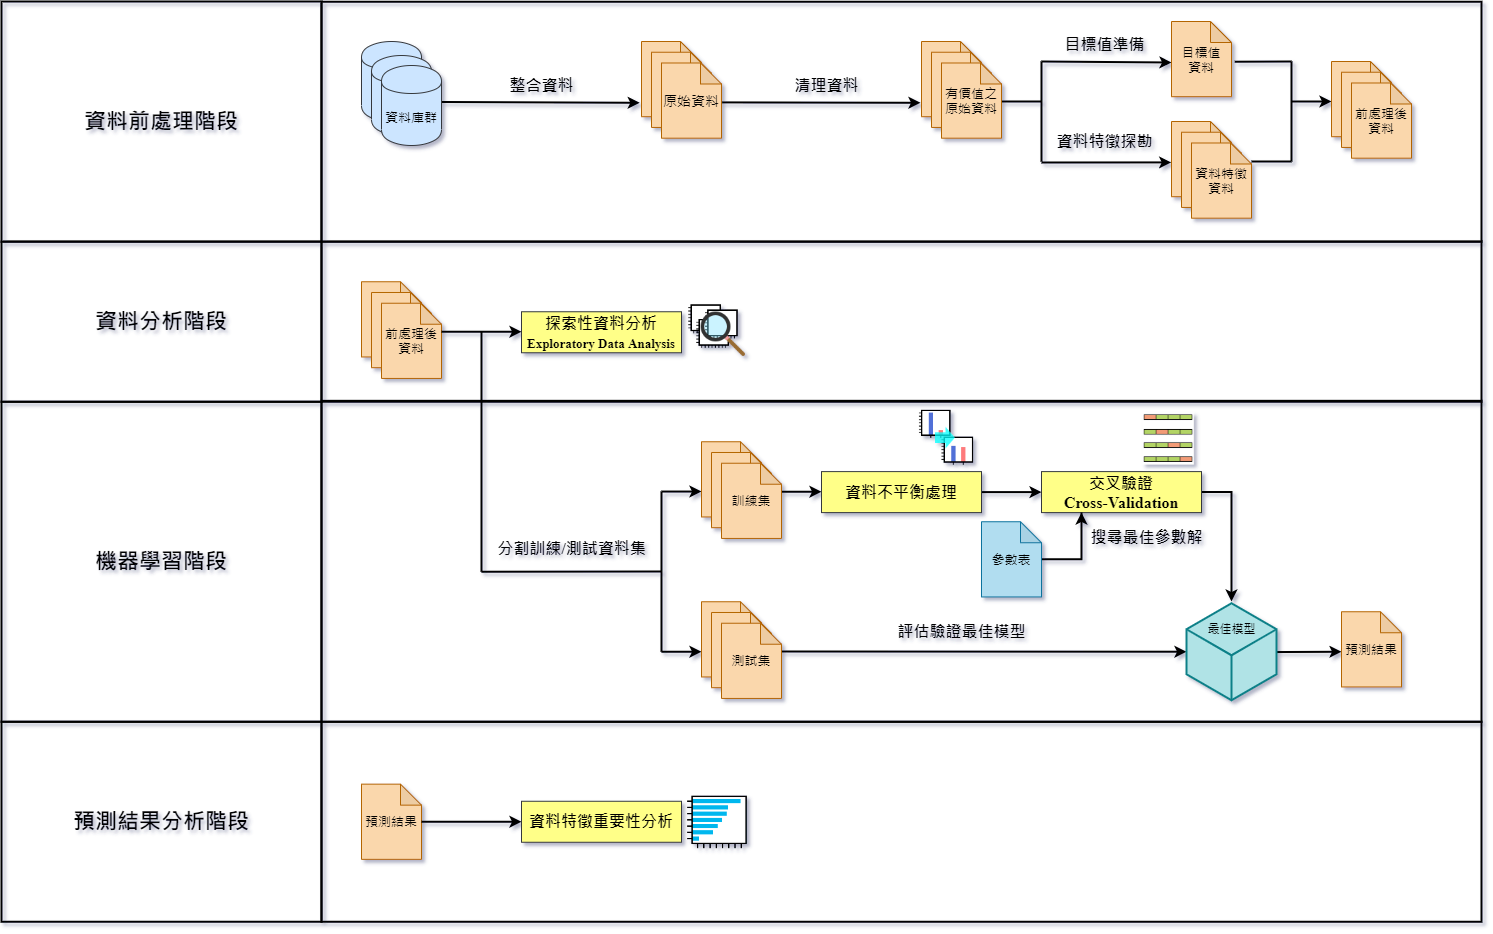
\includegraphics[width=1\textwidth]{figures/Image_Framework.png}
    \caption[本論文之巨量資料探勘框架示意圖]{本論文之巨量資料探勘框架示意圖}
    \label{fig:Image_Framework}
  \end{center}
\end{figure}
\newpage

\section{資料前處理階段}

此階段將著重於資料之整合與過濾,為求能收集到有價值之原始資料,以提高後續分析研究之價值,同時進行目標值的準備、資料特徵的探勘與資料特徵工程,協助機器學習之訓練,目標產出有價值之玩家遊戲行為軌跡資料集。

\subsection{整合資料}

首先資料庫群中之資料皆以天為單位,記錄了各項遊戲之玩家行為軌跡,如圖~\ref{fig:Image_Databases}。此步驟將依各項遊戲為整合目標,重整為多個原始資料集,每個原始資料集中,只會記錄該類遊戲之每位玩家行為軌跡,如圖~\ref{fig:Image_Integration},將可提升後續目標值準備及資料特徵探勘速度。

\begin{figure}[!htb]
  \begin{center}
    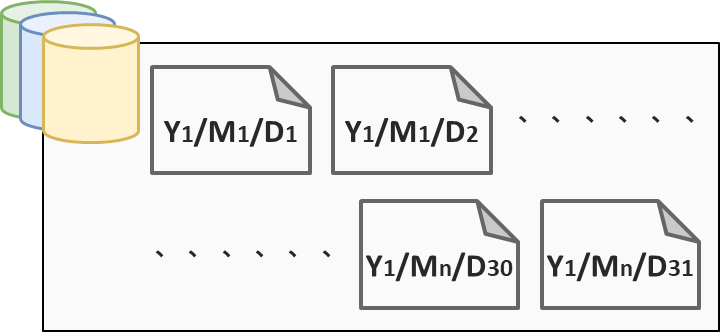
\includegraphics[width=0.7\textwidth]{figures/Image_Databases.png}
    \caption[資料庫群內資料之示意圖]{資料庫群內資料之示意圖}
    \label{fig:Image_Databases}
  \end{center}
\end{figure}

\begin{figure}[!htb]
  \begin{center}
    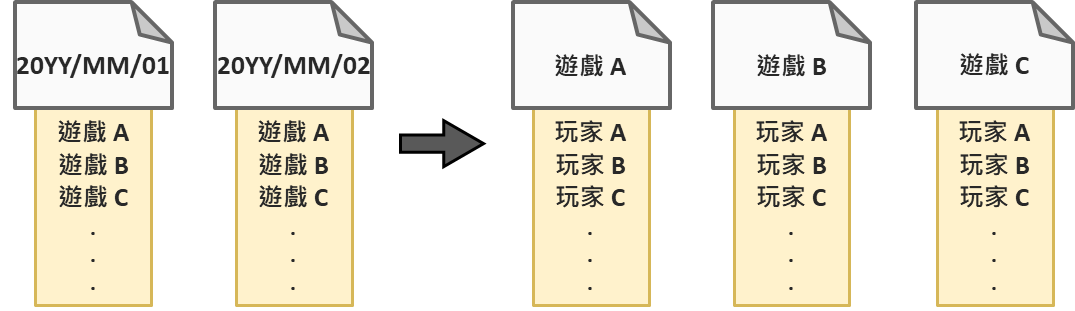
\includegraphics[width=0.9\textwidth]{figures/Image_Integration.png}
    \caption[依各項遊戲為整合目標之示意圖]{依各項遊戲為整合目標之示意圖}
    \label{fig:Image_Integration}
  \end{center}
\end{figure}

除了上述之玩家遊戲行為軌跡原始資料集外,還另外收集了玩家輪廓資料 ( 含國家、玩家等級等 ) 與玩家平台操作紀錄 ( 含消費紀錄、客訴紀錄等 ),最終此步驟將產出三大類原始資料集 (圖~\ref{fig:Image_OriginalDatasets}) :

\begin{itemize}
  \item[■] 玩家輪廓資料 ( 含國家、玩家等級等 )
  \item[■] 玩家平台操作紀錄 ( 含消費紀錄、客訴紀錄等 )
  \item[■] 玩家遊戲行為軌跡
\end{itemize} 

\begin{figure}[!htb]
  \begin{center}
    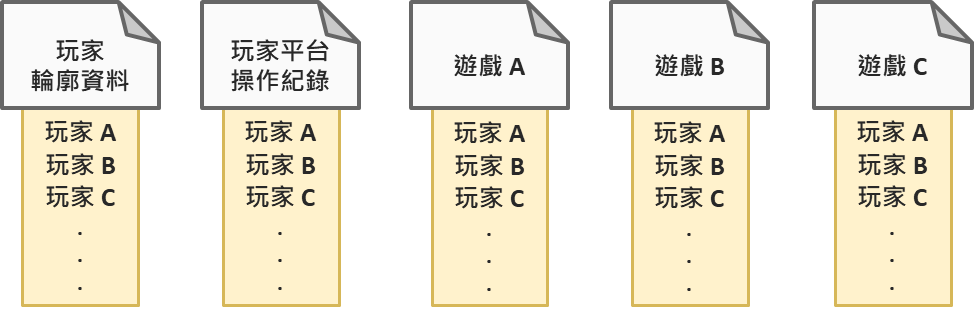
\includegraphics[width=0.8\textwidth]{figures/Image_OriginalDatasets.png}
    \caption[原始資料集示意圖]{原始資料集示意圖}
    \label{fig:Image_OriginalDatasets}
  \end{center}
\end{figure}

\subsection{資料過濾}
\label{subsec:DataFilter}

此步驟將針對兩大議題:刪除空缺值與無價值玩家資料處理。

為了要在資料分析及訓練機器學習時,能夠更加準確的了解及預測真實遊戲玩家之特性與是否流失,需要透過上述之處理,來過濾掉潛在的無用資料,使得整體研究能夠聚焦於更有價值的資料上。

\subsubsection{刪除空缺值}
\label{subsubsec:MissingValueHandle}

為了後續資料特徵重要性分析,希望能保持著資料間的真實性,將採用直接刪去具有空缺值樣本的方式,而不對資料集填入經過處理之假數值,每筆樣本只要在任意資料特徵中擁有一空缺值,即視為欲刪除之對象。

圖~\ref{fig:Image_MissingValueHandle} 為刪除空缺值之示意圖,從圖中可以看出樣本ID 1及2分別在特徵3及1擁有空缺值,將對兩者予以刪除,故最後只留下樣本ID 0及3之資料。

\begin{figure}[!htb]
  \begin{center}
    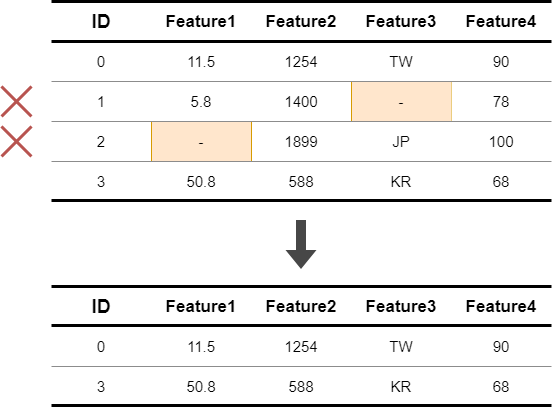
\includegraphics[width=0.8\textwidth]{figures/Image_MissingValueHandle.png}
    \caption[刪除空缺值示意圖]{刪除空缺值示意圖}
    \label{fig:Image_MissingValueHandle}
  \end{center}
\end{figure}

\subsubsection{無價值玩家資料處理}
\label{subsubsec:NonValuePlayerHandle}

對於遊戲領域巨量資料進行研究時,普遍會對所有玩家進行篩檢,以挑選出有價值之玩家族群,可使整體分析與預測更加貼近於真實遊戲情景。定義一時間框架於新進玩家創帳號後,又將其切分為三個時期:

\begin{itemize}
  \item [■] 觀察期:玩家創立帳號後前$O$天。觀察玩家在此時期的行為軌跡,並將對其進行特徵工程,因此,也將觀察期視為資料特徵探勘期。
  \item [■] 挽留期:觀察期之後前$R$天。作為市場操作人員實施挽留策略的時間。
  \item [■] 表現期:挽留期之後前$P$天。決定玩家是否流失,於玩家在觀察期有登入紀錄的前提下,如果玩家在此時期有任一登入紀錄則視為非流失玩家,反之將視為流失玩家。
\end{itemize}

如果該玩家創建帳號的日子較晚,尚未完整擁有上述三個時期的資料,將會造成後續特徵提取與目標值準備的不正確性,進而影響機器學習預測的準確度,因此將其視為無價值玩家,刪除該玩家及其所有行為軌跡。

圖~\ref{fig:Image_DataCleaning} 為判別有價值與無價值玩家之示意圖。從圖中可以看出,玩家1及玩家2已在創帳號後完整經歷觀察期、挽留期與表現期,故視為有價值玩家;而玩家3,因缺少完整的表現期資料,容易被誤判為流失玩家,故視為無價值玩家;玩家4,除了表現期的資料,觀察期資料也並不完整,若將其視為有價值玩家,其錯誤的資料特徵將會影響機器學習之訓練,故也視為無價值玩家。

\begin{figure}[!htb]
  \begin{center}
    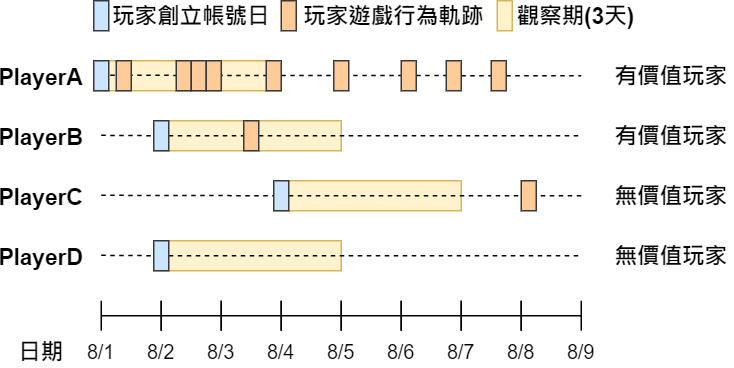
\includegraphics[width=0.9\textwidth]{figures/Image_DataCleaning.png}
    \caption[判別有價值與無價值玩家之示意圖]{判別有價值與無價值玩家之示意圖 (以$O$、$R$、$P$分別為 2、1、2 為例) }
    \label{fig:Image_DataCleaning}
  \end{center}
\end{figure}

經過前兩小節 \ref{subsubsec:MissingValueHandle} 及 \ref{subsubsec:NonValuePlayerHandle} 之處理後,最終此步驟將產出有價值之原始資料集,提供給後續分析及訓練機器學習使用。

\subsection{目標值準備}
\label{subsec:ClassPreparation}

此步驟將準備供機器學習使用之目標值,即為後續預測所需之$class$。定義目標值「非流失玩家」與「流失玩家」,分別代表$class\ 0$及$class\ 1$:

\begin{itemize}
  \item [■] 非流失玩家 ( $class\ 0$ ) :觀察期有登入紀錄的玩家中,表現期間有登入紀錄者,視為非流失玩家。
  \item [■] 流失玩家 ( $class\ 1$ ) :觀察期有登入紀錄的玩家扣除非流失玩家,剩餘者皆為流失玩家;表現期後才有登入紀錄者同樣視為流失玩家。
\end{itemize}

圖~\ref{fig:Image_ClassPreparation} 為定義非流失玩家與流失玩家之示意圖。從圖中可以看出玩家1及玩家2於觀察期及表現期中皆有登入紀錄,故定義為非流失玩家 ( $class\ 0$ ) ;而玩家3及玩家4則在表現期中無登入紀錄,故定義為流失玩家 ( $class\ 1$ ) ,即使玩家4在表現期後有登入紀錄,依舊將其視為流失玩家 ( $class\ 1$ ) 。

\begin{figure}[!htb]
  \begin{center}
    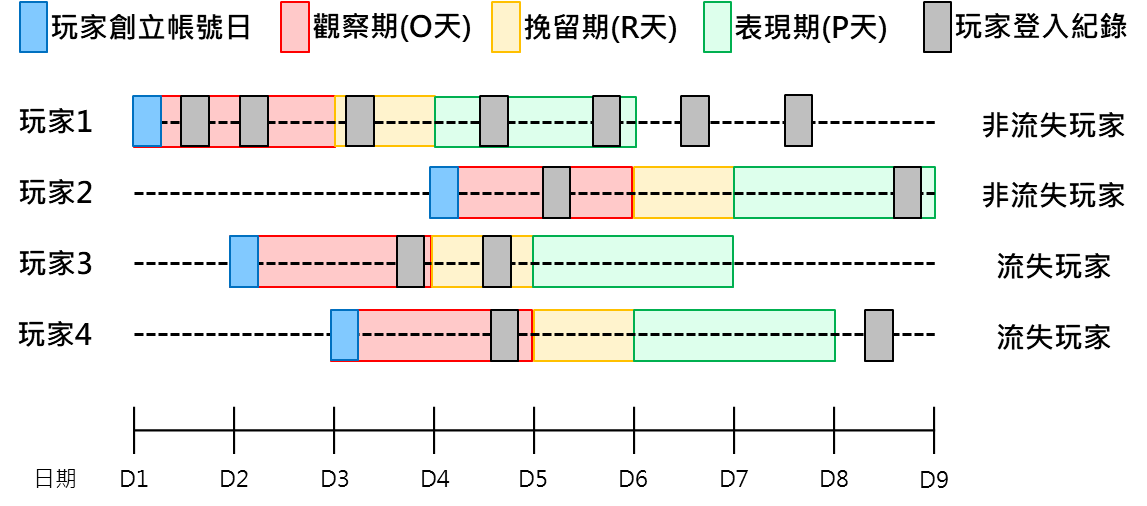
\includegraphics[width=0.9\textwidth]{figures/Image_ClassPreparation.png}
    \caption[非流失玩家與流失玩家之示意圖]{非流失玩家與流失玩家之示意圖 (以$O$、$R$、$P$分別為 2、1、2 為例) }
    \label{fig:Image_ClassPreparation}
  \end{center}
\end{figure}

本論文將預測目標聚焦於流失的新進玩家,所以透過觀察期與表現期來侷限流失玩家之定義。圖~\ref{fig:Image_ClassVennChart} 為流失玩家與非流失玩家范氏圖,可以從圖中看出,最外圍之黑圓框代表所有玩家 (於 \ref{subsubsec:NonValuePlayerHandle}~小節中,篩檢後之有價值玩家) ,而藍色底之圓形範圍代表所有非流失玩家 ( $class\ 0$ ) ,內圈之綠圓框代表前述流失定義門檻,綠圓框內之紅色底圓型範圍則代表所有流失玩家 ( $class\ 1$ ),其中深紅色底之圓形範圍代表表現期後無登入紀錄的玩家;淺紅色底之圓形範圍代表表現期後有登入紀錄的玩家。可以由上述說明來了解到資料內流失玩家與非流失玩家之分佈狀況及其關係。

\begin{figure}[!htb]
  \begin{center}
    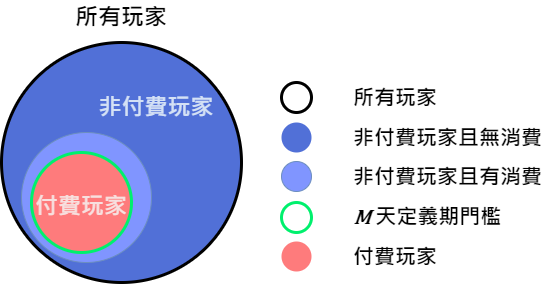
\includegraphics[width=0.6\textwidth]{figures/Image_ClassVennChart.png}
    \caption[流失玩家與非流失玩家范氏圖]{流失玩家與非流失玩家范氏圖}
    \label{fig:Image_ClassVennChart}
  \end{center}
\end{figure}

\subsection{資料特徵探勘與特徵工程}
\label{subsec:FeatureMining}

此步驟將探勘供機器學習使用之資料特徵。在遊戲領域巨量資料中,相較於在學習模型上進行深入研究與改進,透過資料特徵之轉化及選擇顯得更為重要且有效。所以對資料集進行不同面向之探勘,除了可以獲取更多的資訊,也能讓後續資料分析以及機器學習更加順利。

本文將觀察期作為資料特徵探勘期,對每位玩家進行資料特徵探勘,自玩家創立帳號日之$O$天內,探勘其所需之資料特徵。資料特徵之探勘面向將參考於~\cite{sifa2015predicting}~\cite{lee2016predicting}~\cite{martinez2020machine}之探勘想法,主要聚焦於玩家之行為軌跡,並將其進行特徵工程與設計綜合指標特徵。

圖~\ref{fig:Image_FeatureEngineering} 為特徵工程示意圖。紅色箭頭為第一層特徵變數建立方式,對資料集以多種統計方式建立資料特徵,並用多個時間框架做拆分,以獲得第一層特徵變數;藍色箭頭為第二層特徵變數建立方式,針對第一層特徵變數做計算,進一步來得到第二層特徵變數,如變化量特徵等。

\begin{figure}[!htb]
  \begin{center}
    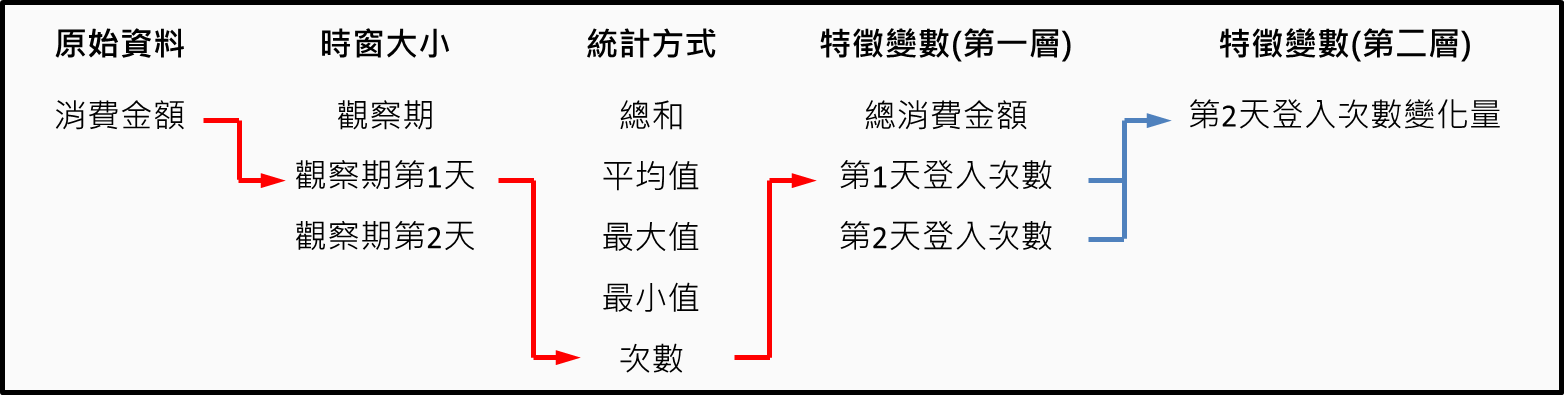
\includegraphics[width=1\textwidth]{figures/Image_FeatureEngineering.png}
    \caption[特徵工程示意圖]{特徵工程示意圖}
    \label{fig:Image_FeatureEngineering}
  \end{center}
\end{figure}

最終可以將資料特徵種類分為三大類:

\begin{itemize}
  \item[■] 玩家輪廓資料:包含玩家自身相關資訊。如創帳號國家、玩家等級等。
  \item[■] 玩家平台操作紀錄:包含玩家以平台為探勘範疇之行為軌跡。如消費紀錄、客訴紀錄等。
  \item[■] 玩家遊戲行為軌跡:包含玩家以遊戲為探勘範疇之行為軌跡。如押注次數、贏分等。
\end{itemize}

%各面向之詳細探勘資料特徵如表~\ref{tab:Features} ,其中遊戲貨幣A及B為購買遊戲內禮包獲得,並為平台內共通之遊戲籌碼。

%\begin{table}[!htb]
%	\centering
%	\begin{tabular}{cclcl}
%		\hline \hline
%		特徵種類 && 特徵 \\
%    \hline \hline
%    \multirow{4}*{玩家資料} && 設備所在地 \\
%    && 設備平台 && \\
%    && 設備廠牌 && \\
%    && 設備型號 && \\
%    \hline
%    玩家平台操作紀錄 && 遊戲貨幣A之餘額變化 \\
%    \hline
%    \multirow{6}*{玩家遊戲行為軌跡} && 遊玩天數 \\
%    && 遊戲貨幣A之餘額變化 \\
%    && 總贏遊戲次數 \\
%    && 總贏分 \\
%    && 獲得遊戲貨幣A之總額 \\
%    && 獲得遊戲貨幣B之總額 \\
%    \hline \hline
%		\end{tabular}
%	\caption[資料特徵種類表]{資料特徵種類表}
%	\label{tab:Features}
%\end{table}
%\newpage

\section{資料分析階段}

此階段將著重於資料的分析。為求在訓練機器學習前,可以藉由資料分析之方法來了解到資料之特性,以提高後續解讀資料特徵之重要性與其相關之連結。另外,還觀察資料特徵是否可以提供給學習模型較多的資訊。

\subsection{探索性資料分析}
採用探索性資料分析,藉由圖表呈現協助了解資料之特性,並且檢查高資訊量之資料特徵,此步驟將利用下列兩種圖表來觀察資料特性:

\begin{itemize}
  \item [■] 長條圖:觀察資料特徵分布情況,如圖~\ref{fig:Image_EDADiagrams} (a)。
  \item [■] 散佈圖:觀察資料特徵間之關聯性,如圖~\ref{fig:Image_EDADiagrams} (b)。
\end{itemize}

\begin{figure}[!htb]
  \centering
  \subfigure[長條圖] {
    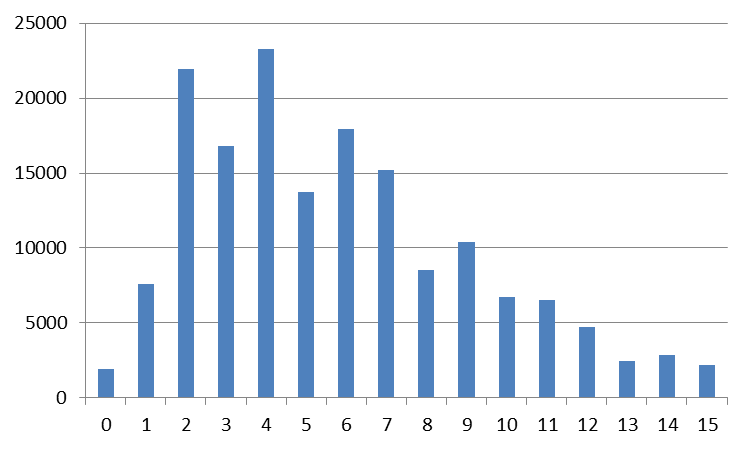
\includegraphics[width=0.45\columnwidth]{figures/Image_BarDiagram.png}
  }
  \subfigure[散佈圖] {    
	  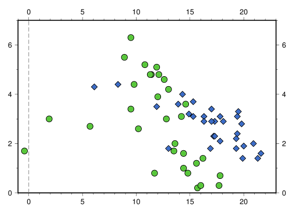
\includegraphics[width=0.45\columnwidth]{figures/Image_ScatterDiagram.png}
  }
  \caption[探索性資料分析之使用圖表類型]{探索性資料分析之使用圖表類型}
  \label{fig:Image_EDADiagrams}
\end{figure}

\subsubsection{高資訊量之資料特徵}
\label{subsubsec:ValuableFeatures}

為了使後續資料特徵重要性之解讀能夠更加清晰,於產出預測結果前即針對資料集進行資料分析,提早推測高資訊量之資料特徵。藉由觀察資料特徵之分佈是否有明顯差異性,而推測此資料特徵能夠提供給學習模型較多的資訊,將此類資料特徵認為是高資訊量之資料特徵,使得後續資料特徵重要性分析之解釋可以更加順利。

%如圖~\ref{fig:Image_ValuableFeatures},可以從圖中看出,非付費玩家資料分佈集中於0附近;而付費玩家資料分佈則分散於y軸上,可見此種資料特徵容易區分出付費玩家與非付費玩家,能夠提供給學習模型較多的資訊。

%\begin{figure}[!htb]
%  \begin{center}
%    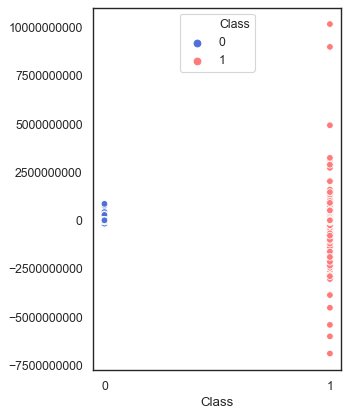
\includegraphics[width=0.45\textwidth]{figures/Image_ValuableFeatures.png}
%    \caption[高資訊量之資料特徵示意圖]{高資訊量之資料特徵示意圖}
%    \label{fig:Image_ValuableFeatures}
%  \end{center}
%\end{figure}

\section{機器學習階段}

此階段將著重於機器學習訓練以及不平衡資料權重調整,最後產出最佳模型之預測結果,提供給流失玩家之預測分析以及資料特徵重要性分析使用。本文選擇樹狀結構之學習模型進行訓練,樹狀結構之學習模型對於巨量資料分類預測顯得更為合適,並且對於預測結果之解釋也相對清楚,而本論文所挑選之學習模型包含:決策樹、隨機森林與極限梯度提升。

\subsection{分割訓練與測試資料集}
\label{subsec:SplitDataset}

透過前述 \ref{subsec:DataFilter}~小節過濾後之資料集,進行訓練集與測試集分割,並按照 $X$:$Y$ 之比例隨機分配。為了避免隨機切割時,目標類別分布不平衡,將採分類隨機抽樣,即流失玩家與非流失玩家各別以 $X$:$Y$ 之比例隨機抽樣,如圖~\ref{fig:Image_SplitDataset}。

\begin{figure}[!htb]
  \begin{center}
    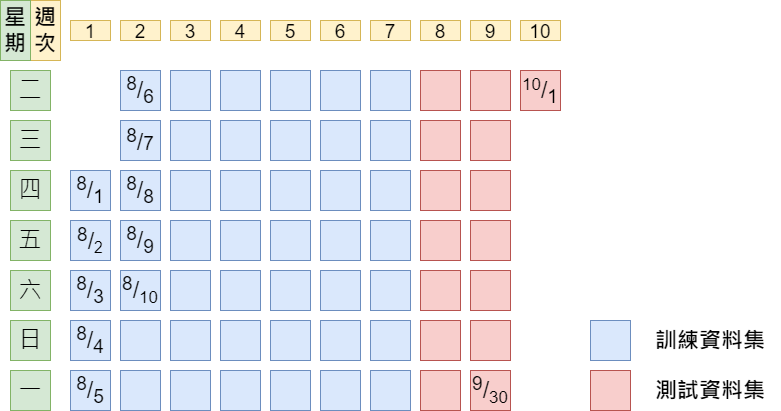
\includegraphics[width=0.8\textwidth]{figures/Image_SplitDataset.png}
    \caption[分割訓練與測試資料集示意圖]{分割訓練與測試資料集示意圖 (以$X$、$Y$分別為 7、3 為例) }
    \label{fig:Image_SplitDataset}
  \end{center}
\end{figure}

\subsection{學習模型選擇}
\label{subsec:ModelSelection}

本文選擇樹狀結構的學習模型進行訓練。樹狀結構的學習模型對於巨量資料分類預測顯得更為合適,並且對於預測結果之解釋也相對清楚,是研究中常使用的學習模型~\cite{wu2008top},因其模型結構能夠清楚表現每筆樣本之預測路徑,可以協助了解到學習模型如何做出決策,如白箱模型 ( white box model );而神經網路結構之學習模型,其模型內的結構難以解析,如黑箱模型 ( black box model ),則無法進行更一步的研究。而本論文所挑選之學習模型包含:

\begin{itemize}
  \item [■] 決策樹:樹狀結構學習模型之最基礎結構,單樹結構,採用CART ( Classification and Regression Tree ) 演算法進行建樹。
  \item [■] 隨機森林:多樹結構,採用裝袋算法建樹。
  \item [■] 極限梯度提升:多樹結構,採用提升方法建樹。
\end{itemize}

上述三種學習模型之資訊量計算以基尼不純度 ( Gini Impurity, $G$ ) 為主,如式~\ref{eq:GiniImpurityFormula},其中$c$為$Class$、$p(i)$為$c$之發生機率。透過基尼不純度 ( $G$ ) 來衡量建樹時之分類準則,挑選出最適合用來進行分割之資料特徵及數值。

\begin{equation}
  \label{eq:GiniImpurityFormula}
  Gini\ Impurity(D) = G(D) = 1 - \sum_{i = 1}^{c}\ p(i)^2
\end{equation}

最後將比較上述三種不同學習模型來挑選出最佳之模型,包含裝袋算法與提升方法不同方式之建樹差異。

\subsection{不平衡資料權重調整}
\label{subsec:ImbalancedDataHandle}

進行機器學習訓練於遊戲領域巨量資料時,往往將會遭受資料不平衡之問題,進而影響學習模型之成效與可靠度。

普遍研究中將針對資料集進行預處理, 設法解決資料不平衡之問題,如SMOTE,為了讓少數群之樣本數與多數群相等,會於原始資料集中放入模擬資料。但本文為了確保資料間之真實性,於處理不平衡資料時,不希望針對資料集進行加工,會無法呈現出真實資料集之特性,所以本文將重點放於訓練學習模型時的樣本權重影響,而不對資料集進行直接處理。樣本權重設置如式~\ref{eq:SampleWeightFormula},其中$N_0$為非流失玩家 ( $class\ 0$ )之樣本數;$N_1$為流失玩家 ( $class\ 1$ )之樣本數。將計算$N_0$與$N_1$之比例差距,此值則為非流失玩家 ( $class\ 0$ )樣本權重放大倍數。

\begin{equation}
  \label{eq:SampleWeightFormula}
%  class\ 0 : class\ 1 = \left \lfloor{\frac{N_1}{N_0}}\right \rfloor : 1
  class\ 0 : class\ 1 = \frac{N_1}{N_0} : 1
\end{equation}

\subsection{搜尋最佳參數解}
\label{subsec:TuningBestParams}

此步驟將對前述 \ref{subsec:ModelSelection}~小節挑選之學習模型進行搜尋最佳參數解,以調教出最適合該學習模型之參數。各學習模型之調教參數如表~\ref{tab:ModelParamsTuning},針對各學習模型之結構不同,挑選不同的參數進行最佳化,各參數意義說明如表~\ref{tab:ModelParamsDescription}。

\begin{table}[!htb]
	\centering
	\begin{tabular}{cclclcl}
		\hline \hline
		學習模型 && Decision Tree && Random Forest && XGBoost \\
    \hline \hline
    \multirow{4}*{參數調教} && max\char`_depth && n\char`_estimators && n\char`_estimators \\
    && min\char`_samples\char`_split && max\char`_depth && max\char`_depth \\
    && min\char`_samples\char`_leaf && min\char`_samples\char`_split && \\
    && min\char`_samples\char`_leaf &&&& \\
    \hline \hline
		\end{tabular}
	\caption[學習模型參數調教表]{學習模型參數調教表}
	\label{tab:ModelParamsTuning}
\end{table}

\begin{table}[!htb]
	\centering
	\begin{tabular}{ccl}
		\hline \hline
		參數 && 參數說明 \\
    \hline \hline
    n\char`_estimators && 多樹結構之樹總數 \\
    \hline
    max\char`_depth && 樹狀結構之最大深度限制 \\
    \hline
    min\char`_samples\char`_split && 節點分割之最小樣本數限制 \\
    \hline
    min\char`_samples\char`_leaf && 葉節點之最小樣本數限制 \\
    \hline \hline
		\end{tabular}
	\caption[學習模型參數說明表]{學習模型參數說明表}
	\label{tab:ModelParamsDescription}
\end{table}

\subsection{交叉驗證 ( Cross Validation ) }
\label{subsec:CrossValidation}

針對訓練資料集進行交叉驗證 ( Cross Validation ),並且搭配前頁之參數調教,最後輸出最佳模型。參考了~\cite{brownlee2020imbalanced}中所使用之RepeatedStratifiedKFold方法,其中使用Stratified方式分割,即為在各Fold中,流失玩家與非流失玩家之資料比例將會相等;使用Repeated方式反覆驗證,即為反覆執行上述之交叉驗證。透過上述之分割方式,可以在每次訓練學習模型時,使真實訓練集保持著原始訓練集的流失玩家與非流失玩家比例。

圖~\ref{fig:Image_RepeatedStratifiedKFold} 為RepeatedStratifiedKFold示意圖。可以從圖中看出,首先依照前述 \ref{subsec:SplitDataset}~小節,從所有資料初步分割出原始訓練集與測試集,再針對原始訓練集進行RepeatedStratifiedKFold,進行了兩次的交叉驗證,而每次分割原始訓練集時可以看到淺藍底之真實訓練集與淺橘底之驗證集中的流失玩家與非流失玩家比例與原始測試集相等,並且真實訓練集與驗證集中的流失玩家與非流失玩家比例也相等。

\begin{figure}[!htb]
  \begin{center}
    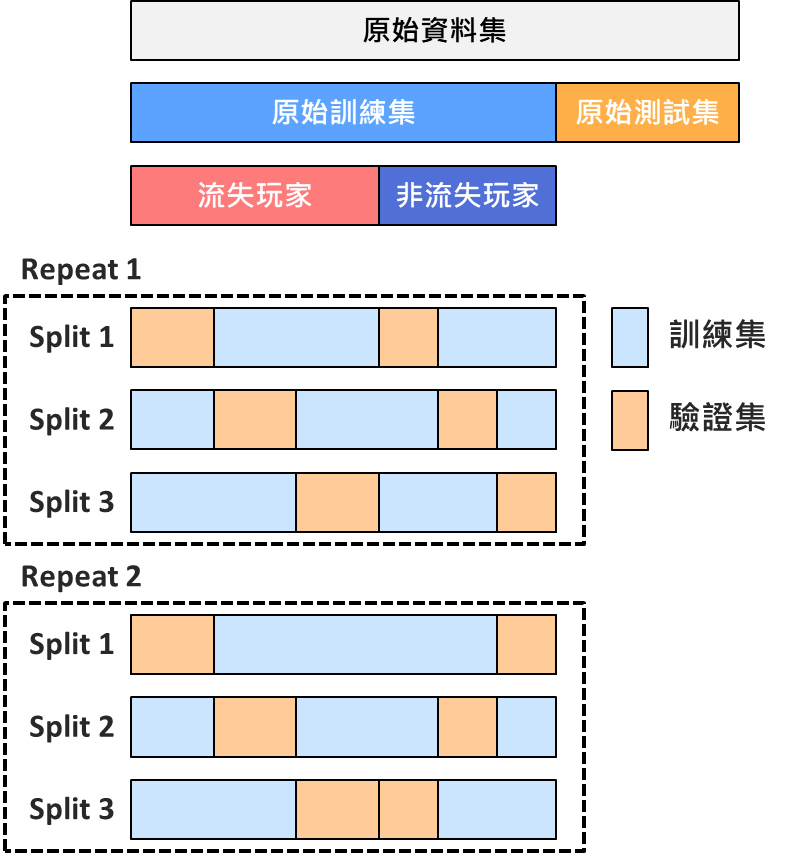
\includegraphics[width=0.7\textwidth]{figures/Image_RepeatedStratifiedKFold.png}
    \caption[RepeatedStratifiedKFold示意圖]{RepeatedStratifiedKFold示意圖 (以Repeated、KFold分別為 2、3 為例) }
    \label{fig:Image_RepeatedStratifiedKFold}
  \end{center}
\end{figure}

%另外,因類別型資料特徵不適用於樹狀結構之學習模型,故在其應用於機器學習前,將此類資料特徵透過One Hot Encoding進行轉化,以利機器學習訓練。

\subsection{評估驗證最佳模型}
\label{subsec:EvaluateBestModel}

前述 \ref{subsec:CrossValidation}~小節中,交叉驗證搭配 \ref{subsec:TuningBestParams}~小節中的參數調教表所使用之評估值為 Weighted F$_{\beta}$ - Score,擇其最高值之學習模型,選定為最佳模型。Weighted F$_{\beta}$ - Score 為在 F$_{\beta}$ - Score 評估值上導入樣本數權重概念,如式~\ref{eq:FbetaFormula} 與式~\ref{eq:WeightedFbetaFormula},適合使用在評估資料不平衡之資料集中。

\begin{equation}
  \label{eq:FbetaFormula}
  F_{\beta} = (1 + \beta^2) \times \frac{precision \times recall}{(\beta^2 \times precision) + recall}
\end{equation}

\begin{equation}
  \label{eq:WeightedFbetaFormula}
  Weighted\ F_{\beta} = \frac{N_1}{N_0 + N_1} \times F_{\beta\ 1} + \frac{N_0}{N_0 + N_1} \times F_{\beta\ 0}
\end{equation}

其中 $\beta$ 則為 Precision 與 Recall 之間的比重,如表~\ref{tab:beta}。本論文預測新進玩家是否會流失,將著重於 Recall,即為將所有可能流失的新進玩家預測出來,因為新進玩家有可能是經由廣告吸引而來,而該玩家身上即帶有廣告投放之成本,故希望能將有可能會流失的新進玩家全部預測出來,使得遊戲商能盡可能地保留住所有玩家。

\begin{table}[!htb]
	\centering
	\begin{tabular}{ccl}
		\hline \hline
		$\beta$數值範圍 && 說明 \\
    \hline \hline
    $0 < \beta < 1$ && 評估著重於 Precision \\
    \hline
    $\beta = 1$ && Precision 與 Recall 比重相當 \\
    \hline
    $1 < \beta$ && 評估著重於 Recall \\
    \hline \hline
		\end{tabular}
	\caption[$\beta$數值意義表]{$\beta$數值意義表}
	\label{tab:beta}
\end{table}

\section{預測結果分析階段}

此階段將著重於資料特徵重要性之分析。透過前述 \ref{subsec:EvaluateBestModel}~小節所產出之預測結果,計算其資料特徵於各學習模型中各樹之重要性,並加總後正規化,產出之分析結果將與前述 \ref{subsubsec:ValuableFeatures}~小節中推測之資料特徵進行探討,並藉由最終結果對遊戲中的遊玩體驗進行評估與建議。

將資料特徵重要性 ( Feature Importance, $fi$ ) 定義為加總各樹中各資料特徵於節點分割時所提供之基尼不純度 ( $G$ ) ( 見式~\ref{eq:GiniImpurityFormula} ) ,稱為基尼重要性 ( Gini Importance, $GI$ ),再將其正規化至區間[0,1]中。

式~\ref{eq:GiniImportanceFormula} 為計算樹中各節點之基尼重要性 ( $GI$ ),其中$D_p$為父節點、$N_p$為父節點之樣本數、$D_{left}$為左子節點、$N_{left}$為左子節點之樣本數、$D_{right}$為右子節點、$N_{right}$為右子節點之樣本數。首先計算$D_p$、$D_{left}$及$D_{right}$之基尼不純度 ( $G$ ),並計算$D_{left}$及$D_{right}$之樣本數權重比例,最後將$D_p$之基尼不純度 ( $G$ ) 減去兩權重值。

\begin{equation}
  \label{eq:GiniImportanceFormula}
  Gini\ Importance(D_p) = GI(D_p) = G(D_p) - \frac{N_{left}}{N_p} \times G(D_{left}) - \frac{N_{right}}{N_p} \times G(D_{right})
\end{equation}

式~\ref{eq:SingleTreeFeatureImportanceFormula} 為計算資料特徵於單樹中之重要性,其中$x$為欲求其重要性之資料特徵、$k$為節點分割時所用資料特徵為$x$之所有節點、$l$為樹中所有節點。首先加總所有$k$之基尼重要性 ( $GI$ ),並加總$l$之基尼重要性 ( $GI$ ),最後將其進行正規化計算,落於區間[0,1]中,並總和為1。

\begin{equation}
  \label{eq:SingleTreeFeatureImportanceFormula}
  fi(t,x) = \frac{\sum_{\ k\ \in\ node\ split\ based\ on\ x}GI(D_k)}{\sum_{\ l\ \in\ all\ nodes}GI(D_l)}
\end{equation}

式~\ref{eq:ModelFeatureImportanceFormula} 為計算資料特徵於多樹中之重要性,其中$x$為欲求其重要性之資料特徵、$t$為學習模型中的所有樹、$N_{trees}$為樹總數。首先加總所有$t$中$x$的$fi(t,x)$,並取其平均於$N_{trees}$中,最後即計算出$x$於學習模型內之資料特徵重要性 ( $fi$ ) 。

\begin{equation}
  \label{eq:ModelFeatureImportanceFormula}
  fi(x) = \frac{\sum_{\ t\ \in\ all\ trees}fi(t,x)}{N_{trees}}
\end{equation}

\section{產業應用分析階段}

此階段將著重於建立代理人模型。代理人模型為一種優化方法,當模型較為複雜、計算量較大時,可以用一簡化模型來替代,例如:用決策樹作為極限梯度提升之代理人模型,結構上較為簡單,在解釋玩家流失的行為規則上也較為清楚。
\newpage